\section{Naïve method: the results}
We now consider $k=2$ correlated tasks. In contrast with multi-modal models, where each spike is a modality with its own estimator, the multi-task setting keeps a \emph{single} estimator $\hat{\vect x}$ that must remain good on all the tasks. A first, intuitive method is designed from the multi-task loss
\[
    \mathcal{L}_{\mathrm{MSE}}(\vect x) := \alpha \norm{\rdmmat Y_1 - \vect x\vect x^T}^2_F + \sqrt{1-\alpha^2} \norm{\rdmmat Y_2 - \vect x\vect x^T}^2_F\,,\qquad \alpha \in [0,1].
\]
Its Hessian, $\mathcal{H} = \alpha \rdmmat Y_1 + \sqrt{1-\alpha^2}\, \rdmmat Y_2 - ( \alpha + \sqrt{1-\alpha^2})\rdmmat I$, depends on the data only through the combined observation $\alpha \rdmmat Y_1 + \sqrt{1-\alpha^2}\, \rdmmat Y_2$. As in the single-spike case, the associated spectral method takes the top eigenvector of this observation as estimator. Unlike the single-spike case, there is no reason for this method to be optimal with correlated spikes, as is known for multi-modal inference~\cite{Keup_2025, mergny2025spectralthresholdscorrelatedspiked, tabanelli2025computationalthresholdsmultimodallearning}. It also sees both tasks at the same time, so it is not a continual learning method: it serves as a baseline for the sequential methods of Section~\ref{sec:ewc}.

The detailed computation can be found in Appendix \ref{proof:naive}.
\subsection{Definition of the method}
We define our observation as:
    \begin{equation}
    \rdmmat Y_{naive} := \alpha \rdmmat Y_1 + \sqrt{1-\alpha^2} \cdot \rdmmat Y_2
    \label{eq:2spikes}
    \end{equation}
    \noindent
    with $ \alpha$ the importance factor, giving how important the task $i = 1,2$ is.
\paragraph{Naive method}
For this method, our estimator $\hat{\vect x}$ is given by the top eigenvector of our observation $\rdmmat Y$, and is then $\hat{\vect x} =\vect{u}_1 $.
\[
\boxed{\; \hat{\vect x}_{naive} = \text{Top eigenvector}(\rdmmat Y)\;}
\]
\subsection{Top eigenvalue}
The top eigenvalue of $\rdmmat P$ can be found to be:
\begin{equation}
    \boxed{\;
    \theta_\pm = \frac{a+b}{2} \pm \sqrt{\Big(\frac{a-b}{2}\Big)^2 + ab\,\rho^2}
    \;}
    \qquad
    a = \alpha\lambda_1, \quad b = \sqrt{1-\alpha^2}\,\lambda_2
    \label{eq:eigenvalue_naive}
\end{equation}
with of course $\theta_+ = \theta_1$ and $\theta_- = \theta_2$ the top two eigenvalues. 
\subsection{Top eigenvector}
\paragraph{Overlap of the estimator with the signals.}
Then considering our estimator $\hat{\vect x}_{naive} := \vect u_1$ being the top eigenvector of the observation $\rdmmat Y$. From equation \ref{eq:overlap_signal_k-spikes}, and rewriting $q_1$ and $q_2$, the overlap of the top eigenvector with our signals are:

\begin{equation}
\boxed{
    m_1 := |\langle \hat{\vect x}_{naive}, \vect{x_1}\rangle| \xrightarrow[n\to\infty]{\text{a.s.}} \Bigg \lvert \frac{\theta_+}{a}c_1^+ \Bigg \rvert \; \sqrt{1-\theta_+^{-2}} }
    \qquad
    \boxed{
    m_2 := |\langle \hat{\vect x}_{naive}, \vect{x_2}\rangle| \xrightarrow[n\to\infty]{\text{a.s.}} \Bigg \lvert  \frac{\theta_+}{b}c_2^+  \Bigg \rvert \; \sqrt{1-\theta_+^{-2}} }
    \label{eq:overlap_naive}
\end{equation}
for $\theta_+ > 1$, and $m_1, m_2 \to 0$ for $\theta_+ \le 1$. For some coeficients $c_1^+, c_2^+$:
\[
\big(c_1^+,\, c_2^+\big) = \frac{\big(r,\, 1\big)}{\sqrt{r^2 + 2\rho\, r + 1}},
    \qquad
    r = \frac{\rho\, a}{\theta_+ - a} = \frac{\theta_+ - b }{b \; \rho}.
\]
\subsection{Numerics}
\begin{figure}[H]
    \centering
    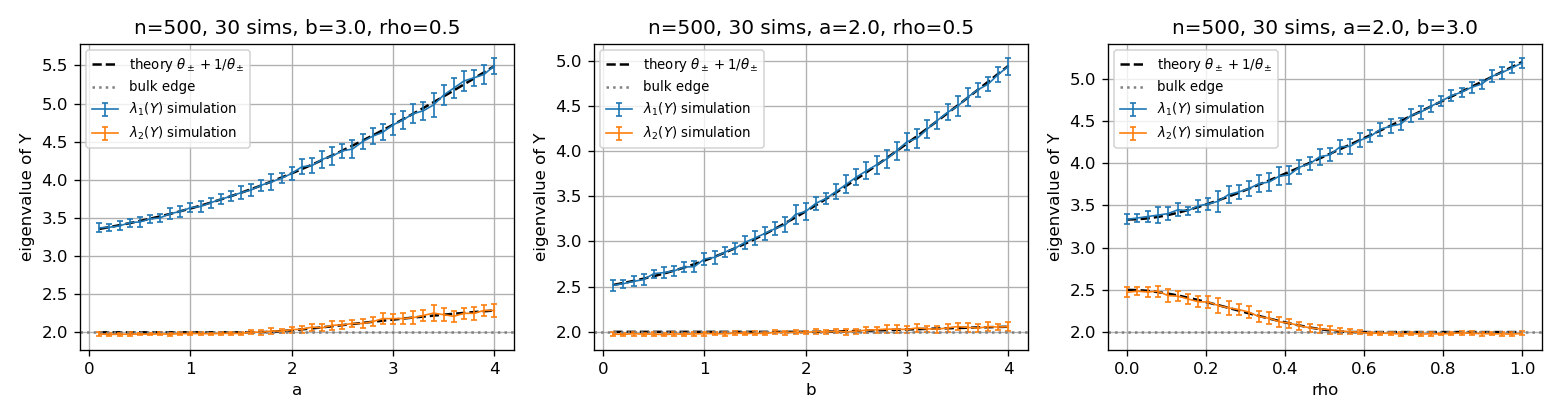
\includegraphics[width=\linewidth]{figures/eigenvalues_Y.png}
    \caption{eigenvalues Y}
    \label{fig:eigenvalues_Y}
\end{figure}




\begin{figure}[ht] 
    \centering 
    \hspace*{-1.3cm}
   \begin{subfigure}{0.3\textwidth}
        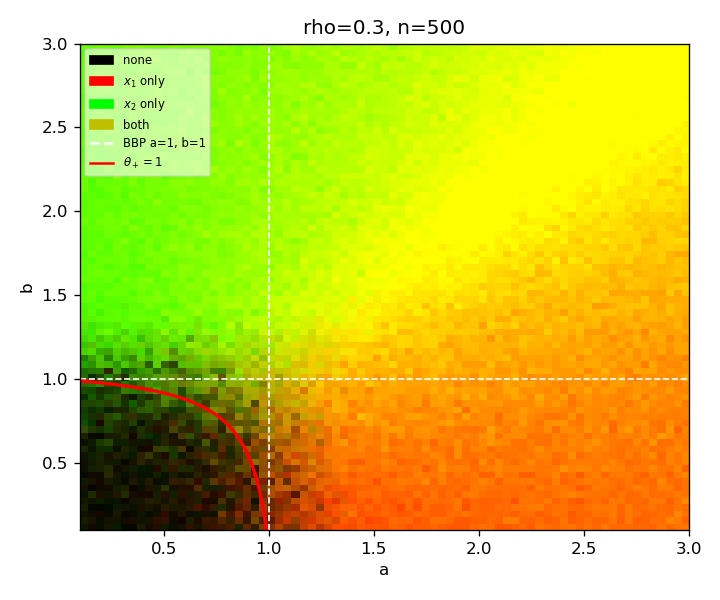
\includegraphics[width=\textwidth]{figures/phase_rho=0.3.png}
                \caption{}

    \end{subfigure}
    \begin{subfigure}{0.7\textwidth}
    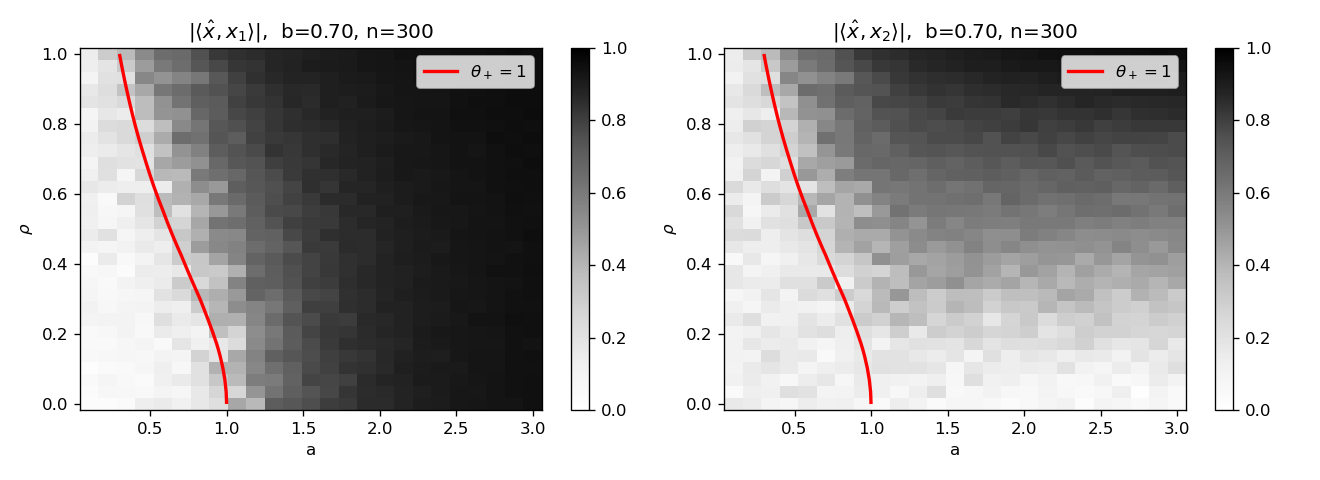
\includegraphics[width=\textwidth]{figures/heat_a_rho.png}
            \caption{}

    \end{subfigure}
  \caption{Recovery thershold}
  \label{fig:overlap_naive}
\end{figure}

\begin{figure}[H]
    \centering
    \includegraphics[width=0.4\linewidth]{figures/overlaps_vs_lambda.png}
    \caption{}
    \label{fig:placeholder}
\end{figure}